\documentclass[a4paper,14pt]{extarticle}
\usepackage[english,russian]{babel}
\usepackage{geometry}
\usepackage[T1]{fontenc}
\usepackage[utf8]{inputenc}
\usepackage{amsmath}
\usepackage{amsthm}
\usepackage{amssymb}
\usepackage{fancyhdr}
\usepackage{setspace}
\usepackage{graphicx}
\usepackage{colortbl}
\usepackage{tikz}
\usepackage{pgf}
\usepackage{subcaption}
\usepackage{listings}
\usepackage{indentfirst}
\usepackage[colorlinks,citecolor=blue,linkcolor=blue,bookmarks=false,hypertexnames=true, urlcolor=blue]{hyperref} 
\usepackage{indentfirst}
\usepackage{mathtools}
\usepackage{booktabs}
\usepackage[flushleft]{threeparttable}
\usepackage{tablefootnote}

\usepackage{chngcntr} % нумерация графиков и таблиц по секциям
\counterwithin{table}{section}
\counterwithin{figure}{section}

\graphicspath{{graphics/}}%путь к рисункам

\makeatletter
\renewcommand{\@biblabel}[1]{#1.} % Заменяем библиографию с квадратных скобок на точку:
\makeatother

\geometry{left=2.5cm}% левое поле
\geometry{right=1.5cm}% правое поле
\geometry{top=1.5cm}% верхнее поле
\geometry{bottom=1.5cm}% нижнее поле
\renewcommand{\baselinestretch}{1.5} % междустрочный интервал


\newcommand{\bibref}[3]{\hyperlink{#1}{#2 (#3)}} % biblabel, authors, year
\addto\captionsrussian{\def\refname{Список литературы (или источников)}} 

\renewcommand{\theenumi}{\arabic{enumi}}% Меняем везде перечисления на цифра.цифра
\renewcommand{\labelenumi}{\arabic{enumi}}% Меняем везде перечисления на цифра.цифра
\renewcommand{\theenumii}{.\arabic{enumii}}% Меняем везде перечисления на цифра.цифра
\renewcommand{\labelenumii}{\arabic{enumi}.\arabic{enumii}.}% Меняем везде перечисления на цифра.цифра
\renewcommand{\theenumiii}{.\arabic{enumiii}}% Меняем везде перечисления на цифра.цифра
\renewcommand{\labelenumiii}{\arabic{enumi}.\arabic{enumii}.\arabic{enumiii}.}% Меняем везде перечисления на цифра.цифра

\usepackage{listings}
\usepackage{color}

\definecolor{dkgreen}{rgb}{0,0.6,0}
\definecolor{gray}{rgb}{0.5,0.5,0.5}
\definecolor{mauve}{rgb}{0.58,0,0.82}

\lstset{frame=tb,
  language=C++,
  aboveskip=3mm,
  belowskip=3mm,
  showstringspaces=false,
  columns=flexible,
  basicstyle={\small\ttfamily},
  numbers=left,
  numberstyle=\color{gray},
  keywordstyle=\color{blue},
  commentstyle=\color{dkgreen},
  stringstyle=\color{mauve},
  breaklines=true,
  breakatwhitespace=true,
  tabsize=2,
  captionpos=b
}


\begin{document}
\begin{titlepage}
\newpage

{\setstretch{1.0}
\begin{center}
Федеральное государственное автономное образовательное учреждение высшего образования «Национальный исследовательский университет «Высшая школа экономики»
\\
\bigskip
Факультет компьютерных наук \\
Основная образовательная программа \\
Прикладная математика и информатика \\
\end{center}
}

\vspace{8em}

\begin{center}
{\Large ВЫПУСКНАЯ КВАЛИФИКАЦИОННАЯ РАБОТА}\\
\textsc{\textbf{
Программный проект на тему
\linebreak
"Оптимизации алгоритмов стандартной библиотеки C++ и прототипирование нового функцонала для будущих стандартов языка программтрования C++."}}
\end{center}

\vspace{8em}

{\setstretch{1.0}
\hfill\parbox{16cm}{
\hspace*{5cm}\hspace*{-5cm}Выполнил студент группы 196, 4 курса,\\
Шитов Александр Андреевич\\
 
\hspace*{5cm}\hspace*{-5cm}Руководитель ВКР:\\
эксперт разработчик Полухин Антон Алексеевич\\

%\hspace*{5cm}\hspace*{-5cm}Куратор:\hfill < степень>, <звание>, <ФИО полностью>\\

% \hspace*{5cm}\hspace*{-5cm}Консультант:\\
% научный сотрудник Лобачева Екатерина Максимовна\\
}
}

\vspace{\fill}

\begin{center}
Москва 2023
\end{center}

\end{titlepage}% это титульный лист
\newpage
\setcounter{page}{2}

\newpage
\section*{Аннотация}
\newpage
\section*{Abstract}
\newpage
{
	\hypersetup{linkcolor=black}
	\tableofcontents
}
\newpage
\section{Введение}
\par{C++ -- язык программирования созданный в 1983 датским ученым в области компьютерных наук Бьйорном Страуструпом. Изначально его идеалогия заключалась в том, что требуется дополнить язык C классами для удобства работы в парадигме ООП. В последствии он развивался мнодествами сообществами программистов, что привело к сложности взаимодействия между этими сообществами. В связи с этим в 1998 году было создана группа стандартизации C++ -- WG21. С помощью этой группы(так же именнуемой коммитетом стандартизации или просто коммитетом) был создан первый стандарт -- C++98, описывающий базовый функционал языка.}
\par{Дальнейшие стандарты начали стабильно выходить с 2011 года с периодичностью три года(с тех пор стандарты называются по формату C++\{две последние цифры года\}) и привнесли множество новых фичей<поменять>, таких как: модель памяти, лямбда-функции, модель потоков, реализация классических алгоритмов и многое другое.}
\par{В этой работе мы сфокусировались на совершенствовании стандартной библиотеки поддержки многопоточности. В частности планируется разработать функционал выставления потоку приоритета так, что бы не приходилось создавать отдельный код для всевозможных API, а так же дополнить функцию std::thread::sleep\_for до вида в котором она существует в std::jthread(то есть добавить stop\_token).}
\par{Помимо этого были проанализированы алгоритмы бинарного поиска и сортировки в реализации стандартной библиотеки и найдены способы оптимизировать их.}
\par{В разделе \ref{literature_review} осуществляется краткий обзор источников используемых по всей работе. Затем начинаются разделы который описывают решение тех или иных задач: оптимизация бинарного поиска \ref{binary_search} и сортировки \ref{sort}; создание функционала потоков \ref{thread_priority} и токена сна \ref{sleep_token}.}

\newpage
\section{Обзор существующих решений и литературы}\label{literature_review}
\subsection{Литература}
\subsubsection{Modern hardware}
\subsection{Известные решения}
\subsubsection{QT}
\subsubsection{Boost}

\newpage
\section{Оптимизация бинарного поиска}\label{binary_search}
\par{Бинарный поиск является одним из самых известных и ключевых алгоритмов. Он применяется во множестве задач где мы имеем дело с отсортированными данными, так как он на порядки быстрее чем его аналог линейный поиск.}
\par{Он имеет две версии в стандартной библиотеке -- std::lower\_bound(левый бинарный поиск\footnote{в подпоследовательности одинаковых элементов будет найден первый}), std::upper\_bound(правый бинарный поиск\footnote{в подпоследовательности одинаковых элементов будет найден последний}). Стандарт накладывает сравнительно небольшие ограничения на эти две функции:
\begin{enumerate}
    \item{Сложность алгоритма по времени -- $O(\log n)$, где $n$ -- размер интервала поиска;}
    \item{Сложность по памяти -- $O(1)$;}\label{binary_search::bounds::space_complexity}
    \item{Исходный интервал не должен быть изменен.}\label{binary_search::bounds::immutability}
\end{enumerate}
Под эти требования подходит общеизвестный алгоритм биннарного поиска<ссылка на Кнута или Кормена>. Однако на практике выясняется, что этот алгоритм может работать значительно быстрее, при этом не нарушая существующих требований. 
}
\subsection{Описание оптимизации}
\par{Существует множество вариантов оптимизации бинарного поиска, например:<вставить примеры из modern hardware>
\begin{enumerate}
    \item{}
    \item{}
    \item{}
\end{enumerate}
Однако все они не подходят так как нарушают или требование \ref{binary_search::bounds::space_complexity}, или требование \ref{binary_search::bounds::immutability}. 
}
\par{Но в данной книге еще упоминается оптимизация, значительно ускоряющая реальную скорость выполнения, при этом не влияющая на ассимптотики и не изменяющая сам массив. Эта оптимизация использует линейный поиск на последних этапах бинарного. В виду особенностей кэша процессора и конвейеризация вычисления это будет значительно быстрее. Описание подробностей того, за счет чего происходит выигрыш.}
\subsection{Обоснование работы}
\par{Современные процессоры редко выполняют операции с одним атомом памяти. Чаще всего они стараются вместе с выполнением взять какую-то полезную нагрузку. Например при чтении данных из памяти мы будем читать не один элемент, а всю его кэш линию\footnote{Кэш-линия - это небольшой блок памяти, используемый для хранения часто используемых данных из более медленной памяти, такой как оперативная память. Кэш-линия обычно имеет фиксированный размер и хранит не больше нескольких десятков байт}. Что касается выполнения инструкций, то при последовательном выполнении одинаковых инструкций процессор может заранее выполнить какие-то инструкции(например с помощью векторизации вычислений\footnote{Векторизация вычислений - это метод оптимизации заключающийся в замене последовательности операций с отдельными элементами данных на операции над векторами данных, то есть наборами элементов, обрабатываемыми одновременно.}). Таким образом мы сможем ускорить проверку внутри цикла когда заранее известно какой элемент будет рассмотрен следующим(то есть нет выбора). Однако наше улучшение не воздействует на бинарный поиск на любых данных -- ввиду того, что функция сравнения двух элементов может изменять внешнее состояние, введя линеаризацию мы можем изменить ожидаемое поведение. Для того, что бы обойти это ограничение мы специализировали нашу функцию на бинарном поиске среди элементов арифметического типа и использующих стандартный компаратор. Благодаря тому, что C++ не позволяет переопределить операторы сравнения для стандартный типов мы можем быть уверены, что наше изменение не повлияет на внешние данные. 
}
\begin{figure}[t]
\begin{lstlisting}[caption={Предложенное изменения бинарного поиска}, label={listing::binary_search}]
  template<typename Iter, typename T, typename Compare>
  typename std::enable_if<std::is_arithmetic<T>::value && (
           std::is_same<Compare, std::greater<T>>::value ||
           std::is_same<Compare, std::less<T>>::value), Iter>::type 
  lower_bound(Iter begin, Iter end, const T& val, Compare comp) {
    constexpr size_t binsearch_distance = std::hardware_constructive_interference_size / sizeof(T); 
    typedef typename std::iterator_traits<Iter>::difference_type _DistanceType;
    _DistanceType len = std::distance(begin, end);
    while (len > binsearch_distance) {
      _DistanceType half = len >> 1;
      Iter middle = begin;
      std::advance(middle, half);
      if (comp(*middle, val)) {
        begin = middle;
        ++begin;
        len = len - half - 1;
      } else {
        len = half;
      }
    }
    for (auto i = begin ; i != end ; ++i) {
        if (!comp(*i, val)) {
            return i;
        }
    }
    return end;
  }
\end{lstlisting}
\end{figure}
\newpage
Разберем строки на листинге \ref{listing::binary_search}, которые отличаются от оригинального алгоритма
\begin{enumerate}
    \item{Строки 2-4 -- для того, что бы мы смогли специализировать нашу функция нам потребовалось использовать SFINAE\footnote{SFINAE -- substitution failure is not an error, парадигма которая позволяет "отключать" функции при не выполнении каких-то условий на этапе компиляции.} со сложным условием внутри;}
    \item{Строка 6 -- вычисление длины отрезка, начиная с которой исполнение переключится на линейный поиск. \\
    Константа std::hardware\_constructive\_interference\_size -- длина кэш-линии в байтах. Поделив длину кэш-линии на размер искомого типа узнаем когда сменить тип поиска(как только длина отрезка станет меньше или равной результату вычисления);}
    \item{Строка 9 -- отличие от оригинала заключается в том, что сравниваем не с 0, а с binsearch\_distance;}
    \item{Строки 21-25 -- цикл линейного поиска, который может быть соптимизирован до векторных операций(зависит от выравнивания данных), но если этого не произойдет то всегда будет использован механизм конвейеризации.}
\end{enumerate}
\subsection{Тесты}
Это улучшение позволяет выиграть в бинарном поиске на десятки процентов. Мы проводили исследования меняя несколько параметров: размер интервала поиска, тип переменной, параметр линеаризации. Приведем ниже графики<приведи ниже графики>
\newpage
\section{Оптимизация сортировки}\label{sort}
\par{Сортировка является одним из главных алгоритмов в любой области программирования. И даже сравнительно небольшое ускорение приведет к существенной оптимищзации утилизации ресурсов. Мы же смогли ускорить алгоритм сортировки в библиотеке GCC для определенных типов данных на порядок -- было $O(n\log n)$ стало $O(n)$. }
\subsection{Описание оптимизации}
\par{У сортировки в стандарте есть несколько ограничений
\begin{enumerate}
    \item{Сортировка должна быть стабильной\footnote{Сортировка является стабильной когда равные элементы в изначальном массиве сохраняют порядок в отсортированном.}}
    \item{Сложность по времени -- $O(n\log n)$}
    \item{Сложность по памяти -- $O(1)$}\label{sort::req::memory}
\end{enumerate}
Исходя из этих требований, например, невозможно добавить сортировку сравнениями(это нарушит требование \ref{sort::req::memory}). Однако мы нашли способ как ускорить сортировку.}
\par{Если посмотреть на то как сортируются типы данных с крайне ограниченым диапозоном значений(например bool), то мы увидим большое количество ненужных действий, что повлияет на итоговую сложность по времени. Однако если мы специализируем нашу сортировку для такого типа данных, и запустим вместо него функцию std::partition\footnote{std::partition -- функция разделения массива данных на две части по результату унарного предиката. Сложность по времени $O(n)$} то сможем существенно выиграть.}
\par{Встает резонный вопрос -- кому может понадобиться отсортировать массив булевых значений? Действительно это используется крайне редко, однако сортировка какого-то массива структур по одному из полей с типом bool явление куда более частое<Можно ли найти пример в опенсорс или сослаться на голые данные яндекса>. Таким образом перед нами появляется последняя проблема -- понять что мы сортируем булевые значения. Во время нашего исследования мы не смогли решить это средствами C++17 и старше. Однако в новой библиотеке алгоритмов std::ranges у сортировки появилась возможность выбрать проекцию -- поле внутри структуры по которому будет выполняться сортировка. Специализирую этот тип мы получим возможность существенно ускорить алгоритм. С помощью спецификатора requires добавленному в C++20 мы можем прописать требования накладываемые на типы данных для спецификации. Здесь помимо требования сортируемости(которое есть и в оригинальном алгоритме) мы добавляем проверку на то, что проекция имеет тип bool.}
\begin{figure}[t]
\begin{lstlisting}[caption={Предложенная спецификация сортировки}, label={listing::sort}]
template<random_access_iterator Iter,
         sentinel_for<Iter> Sent,
         typename Comp = ranges::less,
         typename Proj = identity>
requires sortable<Iter, Comp, Proj> && std::is_same<Proj, bool>
constexpr Iter
operator()(Iter first, Sent last,
           Comp comp = {}, Proj proj = {}) const {
    auto lasti = ranges::next(first, last);
    partition(first, last, __detail::__make_comp_proj(comp, proj));
    return last;
}
\end{lstlisting}
\end{figure}
\subsection{Тесты и примеры}

\newpage
\section{Приоритет потоков}\label{thread_priority}
\subsection{Существующие решения}
\subsection{Значимость работы}
\subsection{Имплементация}

\newpage
\section{Добавление функционала sleep\_token}\label{sleep_token}
\subsection{Существующие решения}
 \subsection{Имплементация}

\newpage
\section{Дальнейшие исследования}\label{future_work}
\newpage
\section{Заключение}\label{conclussion}


\newpage
\section{Примеры} 
\subsection{Ссылки на статьи}

Можно ссылаться на статью вот так:  \bibref{chirkova18}{Chirkova et al.}{2017}.

\subsection{График}

График \ref{fig:by_epochs} достаточно бессмысленный без контекста.

\begin{figure}[h!]
	\centering
	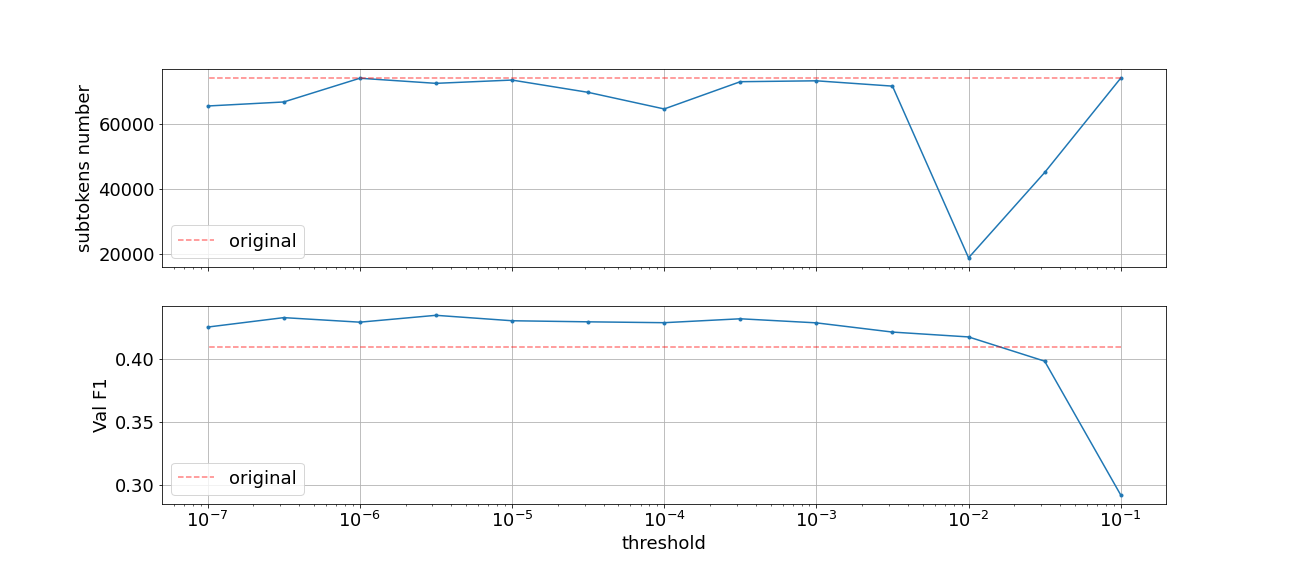
\includegraphics[width=1\textwidth]{example.png}
	\caption{Пример графика}
	\label{fig:by_epochs}
\end{figure}


\subsection{Таблица}

\begin{table}[htbp]
	\caption{Пример таблички}
	\label{table:long_epochs}
	\footnotesize
	\centering
	\begin{tabular}{lrrrrrrrr}
		\toprule
		& \multicolumn{3}{c}{$\mathsf{Val}$} &
		\multicolumn{3}{c}{$\mathsf{Test}$} \\
		\cmidrule(lr){2-4} \cmidrule(l){5-7} 
		{} &  $\mathsf{Prec}$ &  $\mathsf{Rec}$ &  $\mathsf{F1}$ &  $\mathsf{Prec}$ &  $\mathsf{Rec}$ &  $\mathsf{F1}$  &  $\mathsf{nodes}$ & $\mathsf{subtokens}$\\
		\midrule
		запуск 1    &    0.4894 &   0.3775 &  0.4263 &     0.4824 &    0.3683 &   0.4177 & 10029 & 179\\
		запуск 2    &    0.4887 &   0.3739 &  0.4237 &     0.4891 &    0.3724 &   0.4228 & 10039 & 177\\
		запуск 3    &    0.4820 &   0.3751 &  0.4219 &     0.4838 &    0.3677 &   0.4178 & 10037&	180\\
		\midrule
		\bf{среднее} &    \bf{0.4867} &   \bf{0.3755} &  \bf{0.4239} &    \bf{ 0.4851} &    \bf{0.3695} &   \bf{0.4195} \\
		\bf{дисперсия}  &    0.0041 &   0.0019 &  0.0022 &     0.0036 &    0.0025 &   0.0029 \\
		\bottomrule
	\end{tabular}
\end{table}

	
\newpage 

\begin{thebibliography}{0}
\end{thebibliography}
	
\section[A]{Приложение}

\end{document}
